\section{Functionals}
\label{appendix: Functional derivatives}


The principle of stationary action and the path integral method relies on functional calculus, where ordinary, $n$-dimensional calculus is generalized to an infinite-dimensional calculus on a space of functions.
A functional, $S$, takes in a function $\varphi(x)$, and returns a real number $S[\varphi]$.
We will be often be dealing with functionals of the form
%
\begin{equation}
    \label{general action functional}
    S[\varphi] = \int_\Em \dd^n x \, \Ell[\varphi](x),
\end{equation}
%
Here, $\Ell[\varphi](x)$, the Lagrangian density, is a functional which takes in a function $\varphi$, and returns a real number $\Ell[\varphi](x)$ \emph{for each point} $x \in \Em$.
$\Ell$ thus returns a real-valued function, not just a number.
$\Em$ is the manifold, in our case space-time, of which both $\varphi(x)$ and $\Ell[\varphi](x)$ are functions.
The function $\varphi$ can, in general, take on the value of a scalar, complex number, spinor, vector, etc\dots, while $\Ell[\varphi](x)$ must be a scalar-valued function.
This strongly constraints the form of any Lagrangian and is an essential tool in constructing quantum field theories.
Although this section is written with a single scalar-valued function $\varphi$, this can easily be generalized by adding an index, $\varphi \rightarrow \varphi_\alpha$, enumerating all the degrees of freedom, then summing over this index when restating the arguments~\autocite{carrollSpacetimeGeometryIntroduction2019,schwartzQuantumFieldTheory2013,peskinIntroductionQuantumField1995}.



\subsection{Functional derivative}

The functional derivative is base on an arbitrary \emph{variation} $\eta$ of the function $\varphi$.
The variation $\eta$, often written $\delta \varphi$, is an arbitrary function only constrained to vanish \emph{quickly enough} at the boundary $\partial \Em$.\footnote{%
The condition of ``quickly enough'' is to ensure that we can integrate by parts and ignore the boundary condition, which we will do without remorse.
}
The variation of the functional $S$ is defined as
%
\begin{equation}
    \delta_\eta S[\varphi] = \lim_{\epsilon \rightarrow 0} \frac{1}{\epsilon}
    \left( S[\varphi + \epsilon \eta] - S[\varphi] \right) 
    = \odv{}{\epsilon} S[\varphi + \epsilon \eta] |_{\epsilon = 0}.
\end{equation}
%
We can regard the variation of a functional as the generalization of the differential of a function, \autoref{covectors i.e. one forms}, as the best linear approximation around a point.
In regular differential geometry, a function $f$ can be approximated around a point $x$ by
%
\begin{equation}
    f(x + \epsilon v) = f(x) + \epsilon \dd f(v),
\end{equation}
%
where $v$ is a vector in the tangent space at $x$.
In functional calculus, the functional $S$ is analogous to $f$, $\varphi$ to $x$, and $\eta$ to $v$.
We can more clearly see the resemblance by writing
%
\begin{equation}
    \odv{}{\epsilon} f(x + \epsilon v) = \dd f(v) = \pdv{f}{x^\mu} v^\mu.
\end{equation}
%
In the last line we expanded the differential using the basis-representation, $v = v^\mu\partial_\mu$.
To generalize this to functional, we define the \emph{functional derivative}, by
%
\begin{equation}
    \label{definition functional derivative}
    \delta_\eta S[\varphi] = \int_\Em \dd^n x \, \fdv{S[\varphi]}{\eta(x)} \eta(x).
\end{equation}
%
If we let $S[\varphi] = \varphi(x)$, for some fixed $x$, the variation becomes
%
\begin{equation}
    \delta_\eta S [\varphi] = \eta(x) = \int \dd^n y \, \delta(x - y) \eta(y),
\end{equation}
%
which leads to the identity
%
\begin{equation}
    \fdv{\varphi(x)}{\varphi(y)} = \delta(x - y).
\end{equation}
%
There is also a generalized chain rule for functional derivatives.
If $\psi$ is some new functional variable, then
%
\begin{equation}
    \fdv{S[\varphi]}{\varphi(x)}
    = \int_\Em \dd^n y \, 
    \fdv{S[\varphi]}{\psi(y)}
    \fdv{\psi(y)}{\varphi(x)}.
\end{equation}
%
Higher functional derivatives are defined in terms of higher-order variations,
%
\begin{equation}
    \delta^m_\eta S[\varphi]
    = \odv{}{\epsilon} \delta^{m-1}_\eta S[\varphi + \epsilon \eta]|_{\epsilon=0}
    = \int_\Em 
    \left(\prod_{i=1}^m \dd^n x_i \, \eta(x_i)\right) 
    \frac{\delta^m S[\varphi]}{\delta \varphi(x_1)...\delta\varphi(x_m)}.
\end{equation}
%
With this, we can write the functional Taylor expansion,
%
\begin{equation}
    S[\varphi_0 + \varphi]
    = S[\varphi_0]
    + \int_\Em \dd^n x \, \varphi(x) \fdv{S[\varphi_0]}{\varphi(x)}
    + \frac{1}{2} \int_\Em \dd^n x \dd^n y \, \varphi(x) \varphi(y) \fdv{S[\varphi_0]}{\varphi(x), \varphi(y)}
    +\dots.
\end{equation}
%
Here, the notation $\fdv{S[\varphi_0]}{\varphi}$ indicate that $S[\varphi]$ is first differentiated with respect to $\varphi$, then evaluated at $\varphi = \varphi_0$~\autocite{peskinIntroductionQuantumField1995,schwartzQuantumFieldTheory2013}.



\subsection{*Gaussian integrals and the stationary phase approximation}

\label{section:gaussian integrals}

\begin{figure}[H]
    \centering
    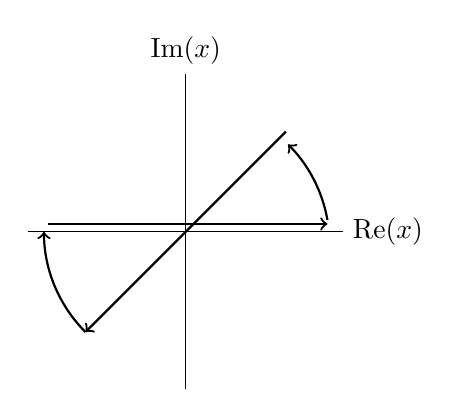
\begin{tikzpicture}
        \draw (-2, 0) -- (2, 0) node[right] {$\mathrm{Re}(x)$};
        \draw (0, -2) -- (0, 2) node[above] {$\mathrm{Im}(x)$};
        \draw[->, thick] (-1.75, 0.1) -- (1.8, 0.1);
        \draw[->, thick] (1.8, 0.15) arc (10:45:1.8);
        \draw[->, thick] ({1.8/sqrt(2)}, {1.8/sqrt(2)}) -- ({-1.8/sqrt(2)}, {-1.8/sqrt(2)});
        \draw[->, thick] ({-1.8/sqrt(2)}, {-1.8/sqrt(2)}) arc (225:180:1.8);
    \end{tikzpicture}
    \caption{Wick rotation}
    \label{Wick rotation}
\end{figure}


An integral that we will use a lot is the Gaussian integral,
%
\begin{equation}
    \int_\R \dd x \, \exp{- \frac{1}{2} a x^2} = \sqrt{\frac{2 \pi}{a}},
\end{equation}
%
for $a \in \R$. The imaginary version,
%
\begin{equation}
    \int_R \dd x \, \exp{i \frac{1}{2} a x^2 }
\end{equation}
%
does not converge. However, if we change $a \rightarrow a + i\epsilon$, the integrand is exponentially suppressed.
%
\begin{equation}
    f(x) = \exp{i \frac{1}{2}a x^2} \rightarrow
    \exp{i\frac{1}{2}a x^2 - \frac{1}{2} \epsilon  x^2}.
\end{equation}
%
As the integrand falls exponentially for $x\rightarrow \infty$ and contains no poles in the upper right nor lower left quarter of the complex plane, we may perform a wick rotation by closing the contour as shown in \autoref{Wick rotation}.
This gives the result
%
\begin{align}
    \label{complex gauss 1D}
    \nonumber
    \int_\R \dd x \, \exp{i \frac{1}{2}(a + i\epsilon) x^2} 
    = \int_{\sqrt{i}\R} \dd x \, \exp{i\frac{1}{2} ax^2} 
    &= \sqrt{i} \int_\R \dd y\, \exp{-\frac{1}{2} (-a) y^2}
    \\ &= \sqrt{\frac{2 \pi i}{(-a)}}
\end{align}
%
where we have made the change of variable $y = (1+i)/\sqrt{2} x = \sqrt{i} x$.
In $n$ dimensions, the Gaussian integral formula generalizes to
%
\begin{equation}
    \int_{\R^n} \dd^n x \, \exp{-\frac{1}{2} x_n A_{nm} x_m } 
    =\sqrt{\frac{(2 \pi)^n}{\det(A)}},
\end{equation}
%
where $A$ is a matrix with $n$ real, positive eigenvalues.
We may also generalize \autoref{complex gauss 1D},
%
\begin{align}
    \int_{\R^n} \dd^n x \, \exp{i\frac{1}{2} x_n( A_{nm} + i \epsilon \delta_{nm}) x_m } =\sqrt{\frac{(2 \pi i )^n}{\det(-A)}}.
\end{align}
%
The final generalization is to functional integrals,
%
\begin{align}
    \nonumber
    \int \D \varphi \, \exp{- \frac{1}{2} \int \dd x \, \varphi(x) A \varphi(x) }
    &= C \det(A)^{-1/2} ,\\
    \int \D \varphi \, \exp{i\frac{1}{2} \int \dd x \, \varphi(x) A \varphi(x) }
    &= C \det(-A)^{-1/2}.
\end{align}
%I
$C$ is here a divergent constant, but will either fall away as we are only looking at the logarithm of $I_\infty$ and are able to throw away additive constants, or ratios between quantities which are both multiplied by $C$.

The Gaussian integral can be used for the stationary phase approximation.
In one dimension, it is
%
\begin{equation}
    \int \dd x \, \exp{i \alpha f(x)} 
    \approx \sqrt{\frac{2 \pi }{f''(x_0)}}\exp{ f(x_0)}, 
    \, \alpha\rightarrow \infty,
\end{equation}
%
where the point $x_0$ is defined by $ f'(x_0) = 0$. 
The functional generalization of this is
%
\begin{equation}
    \int \D \varphi \exp{i S[\varphi]}
    \approx 
    C \det\left(- \frac{\delta^2 S[\varphi_0]}{\delta \varphi^2}\right)
    \exp{i \alpha S[\varphi_0]  },
\end{equation}
%
Here, $S[\varphi]$ is a general functional of $\varphi$, we have used the Taylor expansion, and $\varphi_0$ obeys
%
\begin{equation}
    \fdv{S[\varphi_0]} {\varphi(x)}= 0.
\end{equation}
%





\subsection{The Euler-Lagrange equation}

The Lagrangian may also be written as a scalar function of the field-values at $x$, $\varphi(x)$, as well as its derivatives, $\partial_\mu \varphi(x)$, for example
%
\begin{equation}
    \Ell(\varphi, \partial_\mu \varphi) = \frac{1}{2} \partial_\mu \varphi \partial^\mu\varphi - \frac{1}{2} m^2 \varphi^2 - \frac{1}{4!}\lambda \varphi^4+ \dots.
\end{equation}
%
We have omitted the evaluation at $x$ for the brevity of notation.
We use this to evaluate the variation of a functional in the of \autoref{general action functional}, 
%
\begin{equation}
    \label{variation of action}
    \delta_\eta S[\varphi] = \odv{}{\epsilon}
    \int_\Em \dd^n x \, \Ell[\varphi + \epsilon \eta](x),
\end{equation}
%
by Taylor expanding the Lagrangian density as a function of $\varphi$ and its derivatives,
%
\begin{equation}
    \Ell[\varphi + \epsilon \eta]
    = \Ell
    \left(
        \varphi + \epsilon \eta, \partial_\mu\{\varphi + \epsilon \eta\}
    \right)
     = 
    \Ell[\varphi]
    +
    \epsilon
    \left(
        \pdv{\Ell}{\varphi} \eta 
        + \pdv{\Ell}{(\partial_\mu \varphi)}\partial_\mu\eta 
    \right) + \Oh(\epsilon^2).
\end{equation}
%
Inserting this into \autoref{variation of action} and partially integrating the last term allows us to write the variation in the form \autoref{definition functional derivative}, and the functional derivative is
%
\begin{equation}
    \fdv{S}{\varphi} = \pdv{\Ell}{\varphi} - \partial_\mu \pdv{\Ell}{(\partial_\mu \varphi)}.
\end{equation}
%
The principle of stationary action says that the equation of motion of a field obeys $\delta_\eta S = 0$.
As $\eta$ is arbitrary, this is equivalent to setting the functional derivative of $S$ equal to zero.
The result is the Euler-Lagrange equations of motion~\autocite{schwartzQuantumFieldTheory2013},
%
\begin{equation}
    \pdv{\Ell}{\varphi} 
    -
    \partial_\mu \pdv{\Ell}{(\partial_\mu \varphi)}
    = 0.
\end{equation}




\subsection{Functional calculus on a curved manifold}
\label{subsection: functional calculus on a curved manifold}

As discussed in \autoref{subsection: integration on manifolds}, when integrating a scalar on a curved manifold, we must include the $\sqrt{|g|}$-factor to get a coordinate-independent result.
The action in curved spacetime is therefore
%
\begin{equation}
    S[g, \varphi] = \int_\Em \dd^n x \, \sqrt{|g|} \Ell[g, \varphi],
\end{equation}
%
where the action and the Lagrangian now is a functional of both the matter-field $\varphi$ and the metric $g_{\mu \nu}$.
Our example Lagrangian from last section now takes the form
\begin{equation}
    \label{Lagrangian curved spacetime}
    \Ell(g_{\mu \nu}, \varphi, \nabla_\mu \varphi) = \frac{1}{2} g^{\mu \nu} \nabla_\mu \varphi \nabla_\nu \varphi - \frac{1}{2}m^2 \varphi^2 - \frac{1}{4!}\lambda \varphi^4 \dots,
\end{equation}
%
where partial derivatives are substituted with covariant derivatives.
We define the functional derivative as
%
\begin{equation}
    \delta_\eta S = \int_\Em \dd^n x \sqrt{|g|} \fdv{S}{\eta(x)} \eta(x).
\end{equation}
%
If this is a variation in $\varphi$ only, this gives the same result as before.
However, in general relativity, the metric itself is a dynamic field, and we may therefore vary it.
Consider $g_{\mu \nu} \rightarrow g_{\mu \nu} + \delta g_{\mu \nu}$.
The variation of the action is then
assuming $\Ell$ only depends on $g$ and not its derivatives, we get
%
\begin{equation}
    \label{result derivation of einstein field equation}
    \delta_{g} S = \int_\Em \dd^n x \, 
    \left[
        \left(\delta \sqrt{|g|}\right) \Ell[g] + \sqrt{|g|} \delta \Ell[g]
    \right]
\end{equation}
%
The variation of the $\sqrt{|g|}$-factor can be evaluated using
Using the Levi-Civita symbol $\varepsilon_{\mu_1 \dots \mu_n}$.
The determinant of a $n \times n$-matrix may be written as
%
\begin{equation}
    \det(A) = \frac{1}{n!} \varepsilon_{\mu_1\dots\mu_n}\varepsilon^{\nu_1\dots\nu_n}
    A^{\mu_1}{}_{\nu_1} \dots A^{\mu_n}{}_{\nu_n}.
\end{equation}
%
For a matrix $M$, then, we can write
%
\begin{align}
    \nonumber
    \det(\one + \varepsilon M) &
    = 
    \frac{1}{n!}
    \varepsilon_{\mu_1\dots}\varepsilon^{\nu_1\dots}
    (\one + \epsilon M)^{\mu_1}{}_{\nu_1}  (\one + \epsilon M)^{\mu_2}{}_{\nu_2} \dots\\
    \nonumber
    & =
    \frac{1}{n!}\varepsilon_{\mu_1\dots} \varepsilon^{\nu_1\dots} 
    [
        \delta^{\mu_1}_{\nu_1} \delta^{\mu_2}_{\nu_2} \dots 
        + 
        \epsilon(
            M^{\mu_1}{}_{\nu_1} \delta^{\mu_2}_{\nu_2}\dots 
            + M^{\mu_2}{}_{\nu_2}\delta^{\mu_1}_{\nu_1}\dots 
            +\dots)
    + \Oh(\epsilon^2)]\\
   & 
   = 1 + M^{\mu}{}_{\mu}  + \mathcal{O}(\epsilon^2).
\end{align}
%
Using 
%
\begin{equation}
    \det(g^\mu{}_\nu + \epsilon \eta^\mu{}_\nu)
    =\det(g^\mu{}_\rho[\delta^\rho_\nu + \epsilon g^{\rho\lambda} \eta_{\lambda\nu}])
    = \det(g^\mu{}_\rho) (1  + \epsilon g^{\nu\lambda} \eta_{\lambda\nu}),
\end{equation}
we then get
%
\begin{align}
    \delta \sqrt{|g|}  
    =
    \frac{1}{2}
    \frac{1}{\sqrt{|g|}} \frac{g}{|g|} 
    \delta \det(g)
    = -\frac{1}{2}\sqrt{|g|} g^{\mu \nu} \delta g_{\mu\nu}
\end{align}
%
The minus sign is due to the determinant of a Lorentzian metric being negative. 
Assuming the Lagrangian only depends on the metric directly, and not its derivatives, the variation of the action is
%
\begin{equation}
    \delta_g S
    = 
    \int_\Em \dd^n x \, \sqrt{|g|}
    \left(
       \pdv{\Ell}{g^{\mu\nu}}
    - \frac{1}{2}g_{\mu \nu} \Ell 
    \right) \delta g^{\mu \nu}.
\end{equation}
%
With the Lagrangian in \autoref{Lagrangian curved spacetime}, we get
%
\begin{equation}
    \label{functional derivative with respect to metric}
    \fdv{S}{g^{\mu \nu}}
    =
    \pdv{\Ell}{g^{\mu\nu}}
    - \frac{1}{2}g_{\mu \nu} \Ell 
    =
    - \frac{1}{2}
    \left(
        \frac{1}{2} \nabla_\mu \varphi \nabla_\nu \varphi + \frac{1}{2}m^2 \varphi^2 + \dots
    \right).
\end{equation}
%
We recognize the $(\mu, \nu )= (0, 0)$-component as negative half the Hamiltonian density, which supports the definition of the definition of the stress-energy tensor \autoref{definition stress energy densor}~\autocite{carrollSpacetimeGeometryIntroduction2019}.
 



\subsection{Functional derivative of the Einstein-Hilbert action}
\label{subsection: functional derivative of the einstein-hilbert action}

In the Einstein-Hilbert action, \autoref{Einstein-Hilbert action}, the Lagrangian density is $\Ell = k R = k g^{\mu \nu} R_{\mu \nu}$, where $k$ is a constant and $R_{\mu \nu}$ the Ricci tensor, \autoref{Ricci tensor}.
As the Ricci tensor is dependent on both the derivative and second derivative of the metric, the variation is
%
\begin{equation}
    \delta S_{\text{EH}} = k \int_{\Em} \dd^n x \, \sqrt{|g|}
    \left( \delta R - \frac{1}{2} g_{\mu \nu} R \delta g^{\mu \nu} \right).
\end{equation}
%
The variation of the Ricci scalar is
%
\begin{equation}
    \delta R = R_{\mu \nu} \delta g^{\mu \nu} + g^{\mu \nu} \delta R_{\mu \nu},
\end{equation}
%
We can write the variation of the Ricci scalar, and thus the Riemann curvature tensor, in terms of variations in Christoffel symbols, $\delta \Gamma^{\rho}_{\mu \nu}$ using the explicit formula for a symmetric, metric-compatible covariant derivative, \autoref{riemann tensor in terms of christoffel symbols}.
As $\delta \Gamma = \Gamma - \Gamma'$, it is a tensor, and we may write
%
\begingroup
\allowdisplaybreaks
\begin{align*}
    \delta R^\rho{}_{\sigma \mu \nu} 
    & = \delta(
        \partial_{\mu} \Gamma^\rho_{\nu \sigma} 
        - \partial_{\nu} \Gamma^\rho_{\mu \sigma}
        + \Gamma^\rho_{\lambda \mu} \Gamma^\lambda_{\nu \sigma}
        - \Gamma^\rho_{\lambda \nu} \Gamma^\lambda_{\mu \sigma}
        )\\
    & = \partial_{\mu} \delta \Gamma^\rho_{\nu \sigma} 
        + \Gamma^\rho_{\lambda \mu}\delta \Gamma^\lambda_{\nu \sigma}
        - \Gamma^\lambda_{\mu \sigma}   \delta \Gamma^\rho_{\lambda \nu}
        - \left( 
            \partial_{\nu} \delta \Gamma^\rho_{\mu \sigma} 
            + \Gamma^\rho_{\lambda \nu}\delta \Gamma^\lambda_{\mu \sigma}
            - \Gamma^\lambda_{\nu \sigma} \delta \Gamma^\rho_{\lambda \mu} 
        \right)
        \\ & \quad
        + (\Gamma^{\lambda}_{\mu\nu}\delta\Gamma^\rho_{\lambda \sigma} 
        - \Gamma^{\lambda}_{\mu\nu}\delta\Gamma^\rho_{\lambda \sigma}) \\
    & = \nabla_{\mu}\delta \Gamma^\rho_{\nu \sigma} 
        - \nabla_{\nu}\delta \Gamma^\rho_{\mu \sigma}
     = \nabla_\eta \left(g^\eta{}_{\mu} \delta\Gamma^\rho_{\nu \sigma} 
        - g^\eta{}_{\nu} \delta\Gamma^\rho_{\mu \sigma} \right) 
    := \nabla_\eta K^{\rho\eta}{}_{\mu \rho \nu},
\end{align*}
\endgroup
%
where $K$ is a tensorial quantity, which vanishes at the boundary of our spacetime.
Using the generalized divergence theorem, \autoref{generalized divergence theorem}, we see the contribution to the action from this quantity vanish.
The contribution comes from an integral over $g^{\mu \nu} \delta R_{\mu \nu} = g^{\mu \nu} \delta R^{\rho}{}_{\mu \rho \nu} = g^{\mu \nu} \nabla_\eta K^{\rho\eta}{}_{\mu \rho \nu}$
Using metric compatibility, we can exchange the covariant derivative and the metric, and we have $g^{\mu \nu} \delta R_{\mu \nu} = \nabla_\eta [g^{\mu \nu}K^{\rho \eta}{}_{\mu \rho \nu}]$.
The contribution to the action therefore becomes
%
\begin{equation}
    \int_\Em \dd^4 x \, \sqrt{|g|} g^{\mu \nu} \delta R_{\mu \nu} 
    = \int_\Em \dd^4 x \, \sqrt{|g|} \nabla_\eta K^{\eta \rho \mu}{}_{\rho \mu}
    = \int_{\partial \Em} \dd^3 y \, \sqrt{|\gamma|} n_\eta K^{\eta \rho \mu}{}_{\rho \mu} = 0,
\end{equation}
where we used the fact that $\delta g_{\mu \nu}$, and thus $K$, vanish at $\partial \Em$, and the generalized form of the divergence theorem, \autoref{generalized divergence theorem}.
The variation of the action is therefore
%
\begin{equation}
    \delta S_{\text{EH}} = k \int_\Em \dd^n x \sqrt{|g|} \left[R_{\mu \nu} - \frac{1}{2} R g_{\mu \nu}\right] \delta g^{\mu \nu},
\end{equation}
%
and by the definition of the functional derivative,
%
\begin{equation}
    \label{functional derivatie einstein-hilber action}
    \fdv{S_{\text{EH}}}{g^{\mu \nu}} 
    =
    k(R_{\mu \nu} - \frac{1}{2} R g_{\mu \nu}).
\end{equation}
